\chapter{Plasma sodium, the salt of life}

\section{Plasma sodium, the key player in plasma osmolarity}

Human cells require a tightly regulated extracellular fluid salinity for survival. This regulation is primarily controlled by the osmoregulatory system, which manages water intake and excretion to maintain plasma sodium concentration within a narrow range of 135 to 142 mmol/L, or a more permissive range of 135 to 145 mmol/L.\\

Plasma sodium concentration directly impacts cell volume, with hypernatremia indicating hypertonicity (cell shrinkage) and hyponatremia usually\footnote {This could also be related to hypeglicemic state or pseudohyponatriemia} signifying hypotonicity (cell swelling). Failure to maintain this balance leads to hypotonic or hypertonic stress, exposing cells to potentially dangerous swelling or shrinkage, respectively. This relationship is made possible by the balance between sodium, potassium, and water within the body. While sodium is primarily found in extracellular fluid and potassium intracellularly, their combined concentration in total body water dictates the tonicity of plasma and its effects on cell volume.\\

\section{Tonicity, osmolarity and osmolality: a clarification}
Tonicity, osmolarity, and osmolality are related but distinct concepts often used in physiology, especially when discussing fluid balance and the movement of water between different compartments in the body.\\

Osmolarity refers to the total concentration of solute particles per liter of solution, it is measured in Osmoles per liter (Osm/L). 
\newline In simpler terms it measures the concentration of solutes in a given volume of solvent and does not consider the permeability of a biological membrane nor the type of solute.\\

Osmolality is the total concentration of solute particles per kilogram of solvent, usually water (Osm/kg).
\newline Could be seen as a more accurate measure than osmolarity because it’s not affected by temperature or pressure changes both of which can alter volume. It measures how many solutes are dissolved in a specific weight of solvent, making it particularly useful in biological systems where small variations in fluid volumes matter. In clinical practice for example, blood plasma osmolality is often measured to assess hydration status and is usually around 285-295 mOsm/kg.\\

Tonicity explains the ability of an extracellular solution to generate a water movent in or out of a cell by osmosis, depending on the solute concentration. As it’s a qualitative measure that describes the effect of a solution on cell volume, it has no direct units. 
\newline Tonicity is related to osmolarity but focuses on non-penetrating solutes that can’t cross the cell membrane - also known as effective osmoles - thus affecting water movement and cell volume. When a cell is in a isotonic environment there’s no net movement of water. When a cell is exposed to a lower concentration of non-penetrating solutes compared to the inside (hypotonic fluid), water will move into the cell, causing it to swell. On the contrary, when a cell is exposed to an hypertonic solution, water will move out, causing it to shrink.\\

Sodium (and glucose in cases of insulin deficit), as obligate extracellular solutes acts as effective osmoles and contribute both to osmolality and tonicity, urea in contrast contibutes to osmolality without affecting tonicity as is membrane-permeable.

While water crosses cell membranes freely through aquaporins, solute concentrations (osmolalities) should be equale inside and outside of cells. Na/K-ATPase pump is key in maintaining sodium largely extracellular and postassium mainly intracellular and osmotic gradients are quickly abolished by water movement. This way, the concentration of sodium in the extracellular fluids (ECF) should equale the concentration of sodium plus potassium in total body water (TBW), as described by the Edelman equation \cite{sternsDisordersPlasmaSodium2015a}. So, plasma sodium concentration is influenced both by sodium and potassium balance as well as water balance. Consequently, a noticeable decrease in the total potassium body content will induce a decrease in plasma sodium concentration.	\\

\section{Sodium swings, how the cells adapt over time}
Brain capillaries consist of tight endothelial junctions intertwined by astrocytic foot processes, the so-called blood-brain barrier (BBB), that sodium can't cross and will instead act as an active osmolyte. Consequently, abnormal plasma sodium levels will cause water movement into or out of the brain.\\

Unsurprisingly, since plasma sodium affects brain volume, its regulation is influenced by hypothalamic osmoreceptors in the brain. 
\newline Regulation of serum sodium level is strictly related to water metabolism through antidiuretic hormone (ADH or vasopressin) via the hypothalamic osmostat. Hence plasma sodium concentration responds to changes in water ingested, infused or excreted which can contain large amounts of concentrated salt or could be electrolyte-free water. There are opposing mechanism regulating sodium retention  (sympatethic nervous system and the rening-angiotensin-aldosterone system) and sodium excretion (natriuretic peptides). 
\newline In addition, nonosmotic ADH mechanism are involved. Factors such as hemodynamic instability, pain, drugs (antibiotics, osmolar therapy, opiates) will alter the osmotic threshold for ADH release.
Lastly, we, as clinicians, often restrict fluids intake and the patient in intensive care unit has a suppressed oral intake, making the entire picture even more complex.\\

When changes in plasma sodium occurs the cell adapts to the new state, or at least tries to.\\

After decreases in plasma osmolality, water moves into the brain along osmotic gradients. In response, the brain rapidly loses both extracellular and intracellular solutes (Na+, Cl- and K+). Na+ and Cl- losses begin very rapidly, generally within 30 min, whereas brain K+ losses peak at about 3h. \cite{verbalisBrainVolumeRegulation2010a}\\

Cells contain also organic osmolytes—small intracellular molecules such as glutamate, taurine, and myo-inositol. In a hypotonic state, the cell releases these molecules, while in a hypertonic state, transporters are upregulated to increase their reuptake, with the goal of maintaining minimal changes in cell volume. 
\newline Like many adaptive mechanisms, these processes require time to engage and disengage. If sodium levels change too rapidly, vascular injury can occur due to sudden brain shrinkage, or the brain may swell abruptly, leading to increased intracranial pressure. In some cases, the adaptive mechanisms can make the situation even worse — for example, the release of glutamate may lower the seizure threshold. In general terms the brain is much better at losing organic solutes than to reaccumulate them, in contrast to rapid electrolyte movements (mainly Na+ and Cl-).\\

Astrocytes act as osmotic buffers protecting neurons from osmotic stress by moving taurine and others small molecules. Those changes are within 24 to 48 hours  as the upregulation or down-regulation takes time - if a  sodium turbulence occurs before the new steady state, astrocytes could be osmolyte-depleted and therefore unable to respond properly.\\

This explains why rapid changes in sodium levels must be corrected quickly, before slower adaptive mechanisms based on organic osmoles take effect, and why gradual changes should be managed slowly for the same reason (see fig:1.1). Notably, if the brain is already partially injured, these mechanisms become inefficient and could potentially cause further damage to the salvageable brain tissue \cite{babaApproachManagementSodium2022a}.\\

\begin{figure}[h]
    \centering
    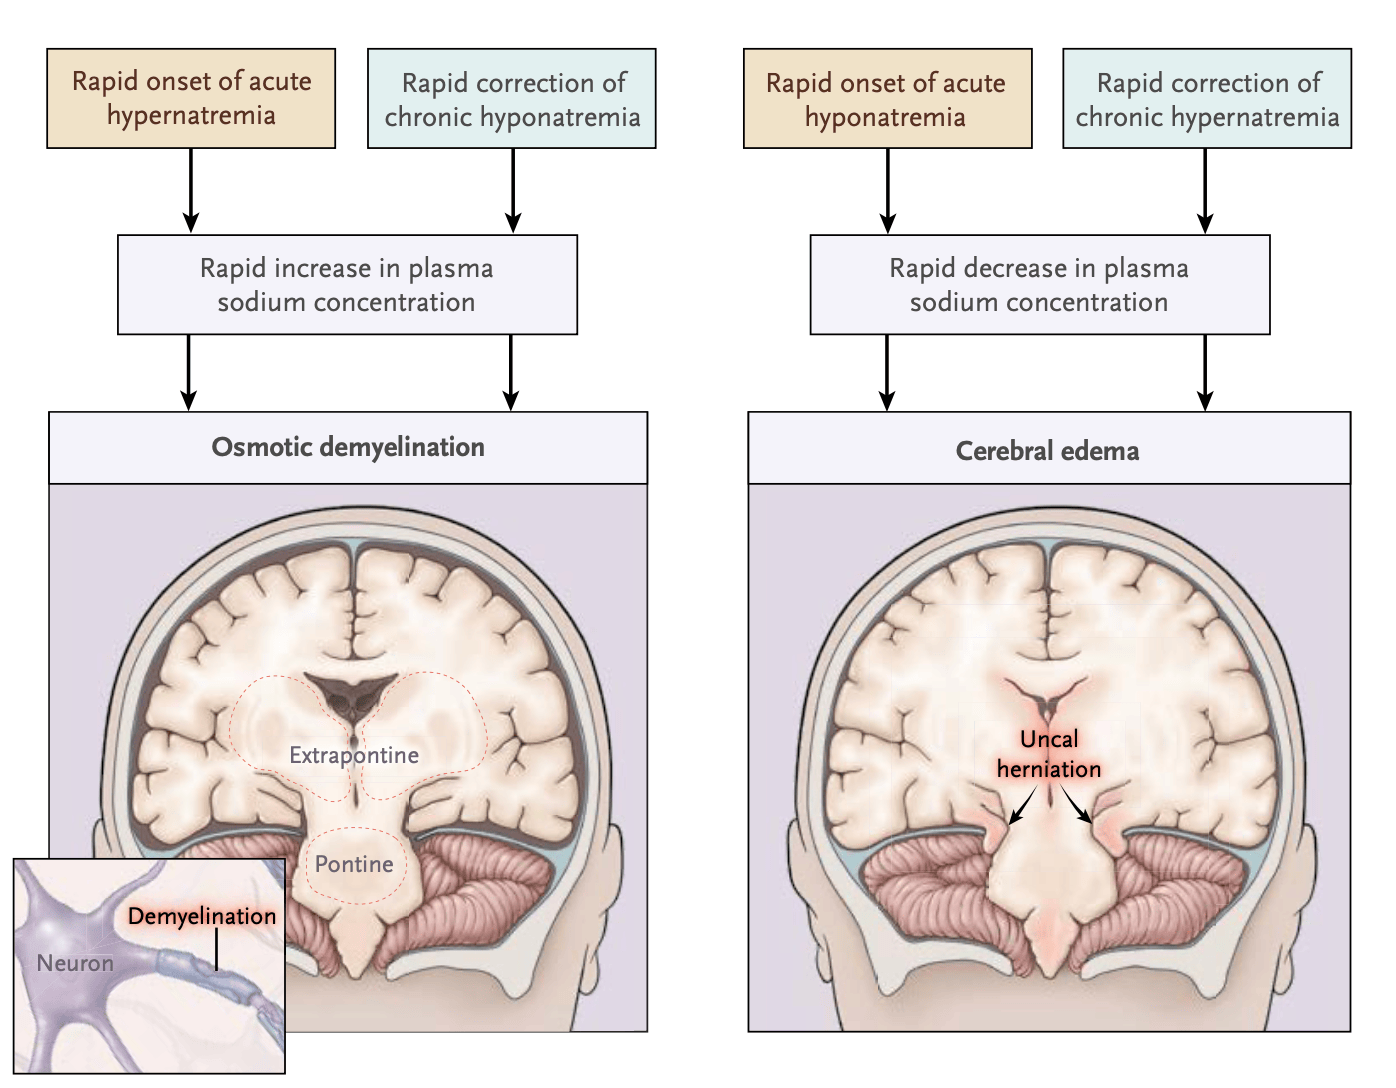
\includegraphics[width=0.8\textwidth]{pictures/fig1.png}
    \caption{Both a rapid onset and a rapid correction of hyponatremia and hypernatremia can cause brain damage. A rapid increase in the level of plasma sodium, either from acute hypernatremia or from rapid correction of chronic hyponatremia, can cause osmotic demyelination. Cerebral edema is a complication of acute hyponatremia and of rapid correction of chronic hypernatremia. Modified from Sterns\cite{sternsDisordersPlasmaSodium2015a}.}
\end{figure}

\section{Salt disruptions, dysnatriemias in the brain injured patient}
Disturbances of plasma sodium concentrations are generally defined as dysnatriemias, those are quite common in the brain injured patient and are associated with poor neurological outcomes and mortality. Brain injury can both induce and result in dysnatriemias.\\

\textbf{Hyponatriemia} is defined as a serum sodium lower than 135 mmol/L. The highest incidence of hyponatriemia is found in subarachnoid hemorrhage (up to 60\% of patients), followed by traumatic brain injury (up to 50\% of patients). The most serious complication is defintely fatal cerebral edema and herniation.
\newline Through aquaporins water moves from the ECF to the intracellular compartment resulting in astrocytic swelling. Water is routed selectively inside glial cells to initially spare the neurons. When placed in a hyposmotic fluid, astrocytes active a mechanism known as \textit {regulatory volume decrease}. The most immediate response consists in the shifting of liquid from the interstitial space to the cerebrospinal fluid. In order to counterbalance the increase in water volume, brain cells rapidly adapt by extruding osmotically active electrolytes, this is a temporary measure as it wanes within a few hours (3 to 12 hours\cite{seayDiagnosisManagementDisorders2020a}\cite{babaApproachManagementSodium2022a}). If hyponatriemia is sustained, a second slower adaptive response begin, based on the efflux of organic solutes. At 48h from hyponatriemia onset, the efflux of inorganic solutes still results in a potentially critical 40\% increase of brain water volume\cite{babaApproachManagementSodium2022a}. The timespan required for the brain to expel more than 90\% of organic osmoles is the physiological basis for discriminating between acute (<48h) and chronic (>48h) hyponatriemia\cite{rafatHyponatremiaIntensiveCare2015a}. 
\newline Altough many conditions can lead to hyponatriemia, in the brain injured those are commonly related to the syndrome of inappropriate release of antidiuretic hormone (SIADH) and cerebral salt wasting syndrome (CSW).
\newline In SIADH, serum antidiuretic hormon levels are erroneously high, resulting in inappropiately elevated urine osmolality secondary to urinary loss of sodium, despite hyponatriemia.
\newline Cerebral sal wasting is primarily a natriuresis problem, thus euvolemia and hypervolemic state are often present in SIADH, wehereas hypovolemia is common in untreated CSW.

At the opposite end of the spectrum, \textbf{hypernatriemia} is defined as serum sodium higher than 145 mmol/L. Glial cells and neurons begin to lose water as a result of the osmotic gradient, while the brain tries to mantain a stable intracellular volume. To protect against  shrinkage, brain moves water from the cerebrospinal fluid into the interstitium, followed by early uptake of ions and late accumulation of organic osmoles. 
\newline In the brain injured patient is common to err on the hypernatriemic state, usually as result of osmotherapy for the management of cerebral edema, though can also be unintended as result of diabetes insipidus or other iatrogenic drugs.
\newline Mannitol induces hypernatriemia by increasing free water loss, while hyperonic saline directly increases plasma sodium.
\newline Central diabetes insipidus (CDI) occurs in case of vasopressin deficit or as a component of the pituitary stalk injury. Hypernatriemia may also manifest as a complication of anterior communicating aneurysm rupture or injury to anterio hypothalamus\cite{mahannaManagementSodiumAbnormalities2015a}.\\

\section[The water wars, understanding SIADH, CSW and DI]{The water wars, understanding SIADH, Cerebral Salt Wasting and Diabetes Insipidus}
In the intricate balance of fluid and electrolyte regulation, three conditions already briefly described stand out for the complex interplay in patients with brain injuries: Syndrome of Inappropriate Antidiuretic Hormone Secretion (SIADH), Cerebral Salt Wasting (CSW), and Diabetes Insipidus (DI), deserving further exploration. 
Together, these conditions represent a “water war” within the body, where misregulation of fluids and electrolytes can quickly escalate to worrisome situations.\\

The \textbf {Syndrome of Inappropriate Antidiuretic Hormone Secretion} (SIADH) - recently renamed as SIAD (syndrome of inappropriate antidiuresis) - is characterized by excessive release of antidiuretic hormone (ADH), leading to water retention and dilutional hyponatremia. This disorder is frequently encountered in neurocritical care patients, particularly following traumatic brain injury (TBI), subarachnoid hemorrhage, and neurosurgical procedures. In SIADH, the kidneys retain free water, resulting in euvolemic hyponatremia with high urine osmolality and sodium concentration. 

The diagnostic criteria include several key markers. Hyponatremia is a hallmark feature, with serum osmolality below 270-275 mOsm, indicating hypotonic plasma. Despite this, urine osmolality is typically elevated, often exceeding 300 mOsm, though values between 100-300 mOsm may place the diagnosis into question. Another important diagnostic feature is high urinary sodium concentration, which suggests that sodium is being excreted despite low plasma sodium levels. Clinically, patients with SIADH appear euvolemic, showing no signs of fluid overload or dehydration. Additionally, the hyponatremia should not be attributable to renal failure, as renal function typically remains intact unless the glomerular filtration rate (GFR) falls below 20-25 ml/min. Common treatments for SIADH involve addressing any reversible causes and promoting adequate protein and salt intake. Fluid restriction to <500-1000 ml/day can be effective in about half of patients, although often difficult.\footnote {Fluid restriction is less likely to succeed if urine osmolality is greater than 500 mOsm or urine sodium exceeds 130 mM.\cite{warrenSyndromeInappropriateAntidiuresis2023}}

For more resistant cases, oral urea is a preferred treatment, and SGLT2 inhibitors have also shown efficacy in clinical trials. Additionally, ADH inhibitors (vaptans) are also used, salt tablets may be an alternative when other treatments are contraindicated.\\

Often confused with SIADH due to overlapping clinical features, \textbf {Cerebral Salt Wasting} (CSW) is distinguished by hypovolemia caused by excessive renal sodium loss. CSW typically occurs in response to brain injury and is associated with high urinary sodium excretion and polyuria. The pathophysiology involves disruption of sympathetic pathways or increased secretion of natriuretic peptides (BNP, ANP), leading to renal salt wasting. The existence of CSW remains controversial, as it can be difficult to distinguish from SIADH due to their similar laboratory profiles. Despite conflicting reports on the prevalence of CSW, evidence suggests it may be linked to aldosterone deficiency in certain patients. Treatment generally includes hypertonic therapy for hyponatremia and isotonic fluids with fludrocortisone to correct hypovolemia, aiming to restore fluid balance. Notably, both CSW and SIADH can be managed with hypertonic saline, although their underlying mechanisms differ\cite{sternsCerebralSaltWasting2008}.\\

In contrast to SIADH and CSW, \textbf {diabetes insipidus} (DI) results from the inability to produce or respond to ADH, leading to excessive water loss and hypernatremia. DI is common in patients with severe brain injury, particularly those involving the hypothalamus or pituitary gland. This condition is marked by polyuria, low urine osmolality, and elevated serum sodium. DI is managed by replacing vasopressin activity with desmopressin (a synthetic ADH analogue) but this  carries the risk of free water retention, which can lead to rebound hyponatremia if not  monitored. A common and effective method to treat hypernatremia is the DDAVP clamp, where a high dose of desmopressin (e.g., 2 mcg IV every 8 hours) is used. However, once hypernatremia is controlled, the dose should be reduced to allow some free water excretion, thus avoiding hyponatremia\cite{macmillanDesmopressinPreventRapid2015}.\\

While SIADH, CSW, and DI all affect sodium and water balance, the primary difference lies in their impact on volume status. SIADH presents with euvolemia, CSW with hypovolemia, and DI with hypovolemia and hypernatremia. Early and accurate diagnosis is crucial in tailoring treatments to the specific disorder, as each requires a vastly different approach—fluid restriction for SIADH, fluid and salt repletion for CSW, and hormone replacement for DI. Failure to distinguish between these conditions can result in improper treatment, exacerbating brain injury and worsening outcomes.

%USARE ARTICOLO Approach to the Management of Sodium Disorders in the Neuro Critical Care Unit